% Options for packages loaded elsewhere
\PassOptionsToPackage{unicode}{hyperref}
\PassOptionsToPackage{hyphens}{url}
%
\documentclass[
]{article}
\usepackage{amsmath,amssymb}
\usepackage{lmodern}
\usepackage{iftex}
\ifPDFTeX
  \usepackage[T1]{fontenc}
  \usepackage[utf8]{inputenc}
  \usepackage{textcomp} % provide euro and other symbols
\else % if luatex or xetex
  \usepackage{unicode-math}
  \defaultfontfeatures{Scale=MatchLowercase}
  \defaultfontfeatures[\rmfamily]{Ligatures=TeX,Scale=1}
\fi
% Use upquote if available, for straight quotes in verbatim environments
\IfFileExists{upquote.sty}{\usepackage{upquote}}{}
\IfFileExists{microtype.sty}{% use microtype if available
  \usepackage[]{microtype}
  \UseMicrotypeSet[protrusion]{basicmath} % disable protrusion for tt fonts
}{}
\makeatletter
\@ifundefined{KOMAClassName}{% if non-KOMA class
  \IfFileExists{parskip.sty}{%
    \usepackage{parskip}
  }{% else
    \setlength{\parindent}{0pt}
    \setlength{\parskip}{6pt plus 2pt minus 1pt}}
}{% if KOMA class
  \KOMAoptions{parskip=half}}
\makeatother
\usepackage{xcolor}
\usepackage[margin=1in]{geometry}
\usepackage{graphicx}
\makeatletter
\def\maxwidth{\ifdim\Gin@nat@width>\linewidth\linewidth\else\Gin@nat@width\fi}
\def\maxheight{\ifdim\Gin@nat@height>\textheight\textheight\else\Gin@nat@height\fi}
\makeatother
% Scale images if necessary, so that they will not overflow the page
% margins by default, and it is still possible to overwrite the defaults
% using explicit options in \includegraphics[width, height, ...]{}
\setkeys{Gin}{width=\maxwidth,height=\maxheight,keepaspectratio}
% Set default figure placement to htbp
\makeatletter
\def\fps@figure{htbp}
\makeatother
\setlength{\emergencystretch}{3em} % prevent overfull lines
\providecommand{\tightlist}{%
  \setlength{\itemsep}{0pt}\setlength{\parskip}{0pt}}
\setcounter{secnumdepth}{-\maxdimen} % remove section numbering
\ifLuaTeX
  \usepackage{selnolig}  % disable illegal ligatures
\fi
\IfFileExists{bookmark.sty}{\usepackage{bookmark}}{\usepackage{hyperref}}
\IfFileExists{xurl.sty}{\usepackage{xurl}}{} % add URL line breaks if available
\urlstyle{same} % disable monospaced font for URLs
\hypersetup{
  pdftitle={Recurrent Neural Network (RNN)},
  pdfauthor={Chirag Shivakumar 1004996, Tan Zen Sheen 1005650},
  hidelinks,
  pdfcreator={LaTeX via pandoc}}

\title{Recurrent Neural Network (RNN)}
\usepackage{etoolbox}
\makeatletter
\providecommand{\subtitle}[1]{% add subtitle to \maketitle
  \apptocmd{\@title}{\par {\large #1 \par}}{}{}
}
\makeatother
\subtitle{Long Short Term Memory Networks (LSTM)}
\author{Chirag Shivakumar 1004996, Tan Zen Sheen 1005650}
\date{2023-04-10}

\begin{document}
\maketitle

\hypertarget{pre-requisites-covered-in-week-3-5}{%
\section{Pre-Requisites (Covered in Week
3-5)}\label{pre-requisites-covered-in-week-3-5}}

\begin{enumerate}
\def\labelenumi{\arabic{enumi}.}
\tightlist
\item
  Neural Networks: The Theory behind Neural Networks
\item
  Back Propagation: Working back from output nodes to input nodes.
\item
  Activation Functions: Sigmoid, Hyperbolic, ReLU, Softmax
\end{enumerate}

\hypertarget{what-is-a-recurrence-neural-network}{%
\section{What is a Recurrence Neural
Network?}\label{what-is-a-recurrence-neural-network}}

A Recurrent Neural Network (RNN) is a basic form of neural network
designed to deal with sequential data, such as time series or Natural
Language Processing (NLP).

A RNN, like any other Neural Network, is made up of weights, biases,
layers, and activation functions. A RNN also has an additional
functionality which is the feedback loop. The key principle underlying
RNNs is that they can keep a ``memory'' of prior inputs, allowing them
to make predictions based on both the present and previous inputs.
Thereby, the feedback loop is used to predict sequential input values
over time.

\hypertarget{machine-learning-fundamentals-for-sequential-data}{%
\section{Machine Learning Fundamentals for Sequential
Data}\label{machine-learning-fundamentals-for-sequential-data}}

Let us say that we have a sequential data
\(X = \{ x_{1},x_{2},x_{3},\ldots,\ x_{n}\}\) and we want to use RNN to
``learn'' the pattern of the data to predict future data.

We can use a Timestep of the Data, of length \(T\), to predict the next
\(K\) values in the dataset

\[use\ {\overrightarrow{x}}^{t} = \begin{bmatrix}
x_{t} \\
x_{t + 1} \\
\ldots \\
x_{t + T} \\
\end{bmatrix}\ to\ predict\ {\widetilde{y}}^{t} = \begin{bmatrix}
{\widetilde{x}}_{t + T + 1} \\
{\widetilde{x}}_{t + T + 2} \\
\ldots \\
{\widetilde{x}}_{t + T + k} \\
\end{bmatrix}\]

We can use Moving Averages to do this, however, doing so may cause
results to not be accurate in predicting the next data in the series.

Therefore, for RNN, there is a ``memory element'' that is used in the
prediction, such that the previous data in the sequence affects the
future predictions. Let us call that the hidden vector
\({\overrightarrow{h}}^{t}\).

This ``memory element'' should also store some information about the
prediction \({\widetilde{y}}^{t}\). So we can compute
\({\widetilde{y}}^{t}\) as some linear combination of
\({\overrightarrow{h}}^{t}\).

\begin{figure}
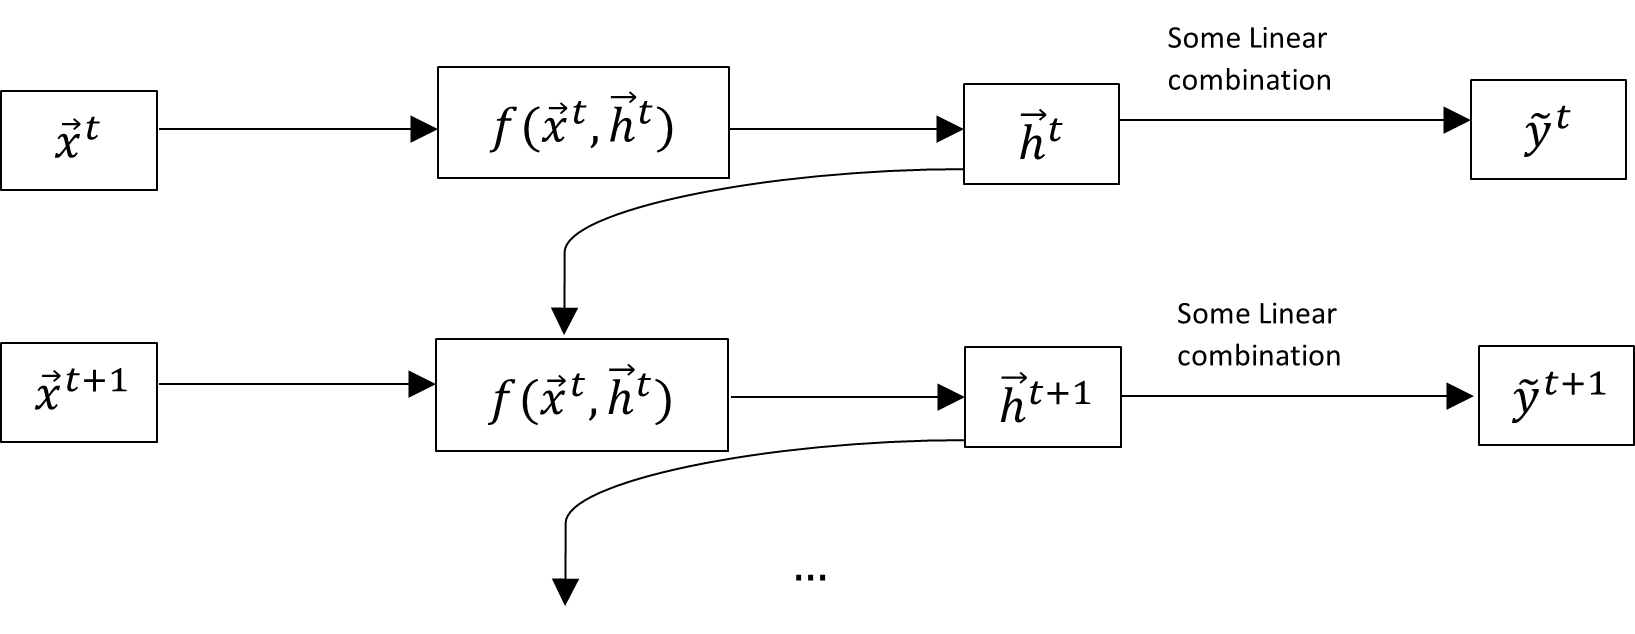
\includegraphics[width=1.5\linewidth]{Simple_Flow} \caption{Simple Flow of RNN}\label{fig:unnamed-chunk-2}
\end{figure}

With this flow in mind, we can construct the recursive equation for the
hidden vector \({\overrightarrow{h}}^{t}\) and the prediction
\({\widetilde{y}}^{t}\) as such:

\[{\overrightarrow{h}}^{t} = f\left( \overline{W}{\overrightarrow{h}}^{t - 1} + \overline{U}{\overrightarrow{x}}^{t} \right),\ \ \widetilde{y} = \overline{V}{\overrightarrow{h}}^{t}\ \]

Where we define the following parameters and vectors

\begin{itemize}
\item
  \({\overline{W}}_{J \times J} \Rightarrow\) Weighing Parameter for the
  previous hidden vector \({\overrightarrow{h}}^{t - 1}\)
\item
  \({\overline{U}}_{J \times T} \Rightarrow\) Weighing Parameter for the
  timestep data \({\overrightarrow{x}}^{t}\)
\item
  \({\overline{V}}_{K \times J} \Rightarrow\) Weighing Parameter for the
  hidden vector \({\overrightarrow{h}}^{t}\) to compute the prediction
  \({\widetilde{y}}^{t}\)
\item
  \({\overrightarrow{x}}^{t}\) \(\epsilon\) \(R^{T} \Rightarrow\)
  Timestep Data
\item
  \({\overrightarrow{h}}^{t}\epsilon R^{J} \Rightarrow\) Hidden Vector
\item
  \({\widetilde{y}}^{t}\epsilon R^{K}\)
\end{itemize}

Dimensional Parameters

\begin{itemize}
\item
  \(T \Rightarrow\) Length of Timestep
\item
  \(K \Rightarrow\) Ouput Dimension
\item
  \(J \Rightarrow\) Dimension of hidden vector
\end{itemize}

Activation function (use sigma function)

\[f(x) = \sigma(x) = \frac{1}{1 + exp( - x)}\]

With this, the Architecture of RNN is as such:

\begin{figure}
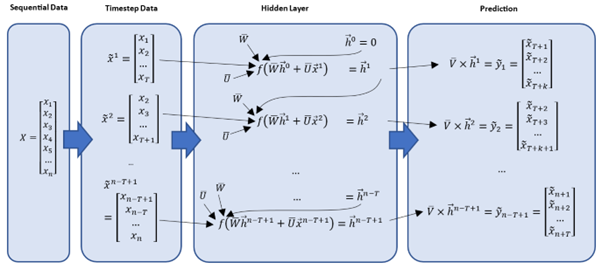
\includegraphics[width=1\linewidth]{RNN_Architecture} \caption{Simple Flow of RNN}\label{fig:pressure}
\end{figure}

Based on the prediction \({\widetilde{y}}^{t}\), we can compute the loss
function from the actual values of\\

\[{\overrightarrow{y}}_{i} = \begin{bmatrix}
x_{t + T + 1} \\
x_{t + T + 2} \\
\ldots \\
x_{t + T + k} \\
\end{bmatrix}\] as follows:

\[L = \frac{1}{2}\sum_{i = 1}^{n - T + 1}\left( {\widetilde{y}}_{i} - y_{i} \right)^{2}\]

In finding the partial derivatives, it is worth noting the derivative of
the sigma function can be simplifies as:

\[f^{'}(x) = \sigma^{'}(x) = \sigma(x)\left( 1 - \sigma(x) \right) = {\overrightarrow{h}}^{t}\left( 1 - {\overrightarrow{h}}^{t} \right)\]

From the loss function, we can thus compute the following partial
derivatives of the weighting parameters,
\(\frac{\partial L}{\partial\overline{W}}\),
\(\frac{\partial L}{\partial\overline{U}}\),
\(\frac{\partial L}{\partial\overline{V}}\):

\[\frac{dL_{i}}{dV_{\alpha\beta}} = \frac{\partial L_{i}}{\partial{\widetilde{y}}_{j}}\frac{\partial{\widetilde{y}}_{j}}{\partial V_{\alpha\beta}} = \left( {\widetilde{y}}_{i} - y_{i} \right)h_{k}\]

\[\frac{dL}{d\overline{V}} = \sum_{i = 1}^{n - T + 1}{\left( {\widetilde{y}}_{i} - y_{i} \right)h_{k}}\]
Equation for Derivative
\[ \frac{dL_{i}}{dU_{\alpha\beta}} = \ \frac{\partial L_{i}}{\partial{\widetilde{y}}_{j}}\frac{\partial{\widetilde{y}}_{j}}{\partial h_{k}}\frac{\partial h_{k}}{\partial U_{\alpha\beta}} \]

\[= \left( {\widetilde{y}}_{i} - y_{i} \right)\left( V_{ij} \right)\left( f^{'}\left( \overline{W}{\overrightarrow{h}}^{t - 1} + \overline{U}{\overrightarrow{x}}^{t} \right) \right)\left( {\overrightarrow{x}}^{i} \right)\]

\[= \left( {\widetilde{y}}_{i} - y_{i} \right)\left( V_{ij} \right)\left( {\overrightarrow{h}}^{t}\left( 1 - {\overrightarrow{h}}^{t} \right) \right)\left( {\overrightarrow{x}}^{i} \right)\]

\[\frac{dL}{dU} = \sum_{i = 1}^{n - T + 1}{\left( {\widetilde{y}}_{i} - y_{i} \right)\left( V_{ij} \right)\left( {\overrightarrow{h}}^{t}\left( 1 - {\overrightarrow{h}}^{t} \right) \right)\left( {\overrightarrow{x}}^{i} \right)}\]

\[\frac{dL_{i}}{dW_{\alpha\beta}} = \frac{\partial L_{i}}{\partial{\widetilde{y}}_{j}}\frac{\partial{\widetilde{y}}_{j}}{\partial h_{k}}\frac{\partial h_{k}}{\partial W_{\alpha\beta}}\]

\[= \left( {\widetilde{y}}_{i} - y_{i} \right)\left( V_{ij} \right)\left( f^{'}\left( \overline{W}{\overrightarrow{h}}^{t - 1} + \overline{U}{\overrightarrow{x}}^{t} \right) \right)\left( \ {\overrightarrow{h}}^{i - 1} \right)\]

\[= \left( {\widetilde{y}}_{i} - y_{i} \right)\left( V_{ij} \right)\left( {\overrightarrow{h}}^{t}\left( 1 - {\overrightarrow{h}}^{t} \right) \right)\left( \ {\overrightarrow{h}}^{i - 1} \right)\]

\[\frac{dL}{dW} = \sum_{i = 1}^{n - T + 1}{\left( {\widetilde{y}}_{i} - y_{i} \right)\left( V_{ij} \right)\left( {\overrightarrow{h}}^{t}\left( 1 - {\overrightarrow{h}}^{t} \right) \right)\left( \ {\overrightarrow{h}}^{i - 1} \right)}\]

Gradient Descent

\[W_{\alpha\beta} \rightarrow W_{\alpha\beta} - \varepsilon\frac{dL}{dW_{\alpha\beta}}\]

\[U_{\alpha\beta} \rightarrow U_{\alpha\beta} - \varepsilon\frac{dL}{dU_{\alpha\beta}}\]

\[V_{\alpha\beta} \rightarrow V_{\alpha\beta} - \varepsilon\frac{dL}{dV_{\alpha\beta}}\]

Algorithm

Initialize Parameters

\begin{itemize}
\item
  \(\overline{W} = 0,\ \overline{V} = 0,\ \overline{U} = 0\)
\item
  \({\overrightarrow{h}}^{0} = 0\ \)
\end{itemize}

Iterate for N epochs

For every n-T+1 combination of
\[{\overrightarrow{x}}^{t} = \begin{bmatrix}
x_{t} \\
x_{t + 1} \\
\ldots \\
x_{t + T} \\
\end{bmatrix}\] ,

Find hidden vector from previous hidden vector\\
\[{\overrightarrow{h}}^{t} = f\left( \overline{W}{\overrightarrow{h}}^{t - 1} + \overline{U}{\overrightarrow{x}}^{t} \right)\]

Compute predictions
\[{\widetilde{y}}_{t} = \overline{V}{\overrightarrow{h}}^{t} = \overline{V}f\left( \overline{W}{\overrightarrow{h}}^{t - 1} + \overline{U}{\overrightarrow{x}}^{t} \right)\ \forall t = 1,\ 2,\ ...n - T + 1\]

Compute Partial Derivatives and update Parameters

\[\frac{dL}{d\overline{V}} = \sum_{i = 1}^{n - T + 1}{\left( {\widetilde{y}}_{i} - y_{i} \right)h_{k}}\]

\[\overline{V} \rightarrow \overline{V} - \varepsilon\frac{dL}{d\overline{V}}\]

\[\frac{dL}{d\overline{U}} = \sum_{i = 1}^{n - T + 1}{\left( {\widetilde{y}}_{t} - y_{t} \right)\left( V_{ij} \right)\left( {\overrightarrow{h}}^{t}\left( 1 - {\overrightarrow{h}}^{t} \right) \right)\left( {\overrightarrow{x}}^{t} \right)}\]

\[\overline{U} \rightarrow \overline{U} - \varepsilon\frac{dL}{d\overline{U}}\]

\[\frac{dL}{d\overline{W}} = \sum_{i = 1}^{n - T + 1}{\left( {\widetilde{y}}_{i} - y_{i} \right)\left( V_{ij} \right)\left( {\overrightarrow{h}}^{t}\left( 1 - {\overrightarrow{h}}^{t} \right) \right)\left( \ {\overrightarrow{h}}^{i - 1} \right)}\]

\(\overline{W} \rightarrow \overline{W} - \varepsilon\frac{dL}{d\overline{W}}\)

\hypertarget{common-types-of-rnn}{%
\subsection{Common types of RNN;}\label{common-types-of-rnn}}

\begin{enumerate}
\def\labelenumi{\arabic{enumi}.}
\tightlist
\item
  One-to-One
\item
  One-to-Many
\item
  Many-to-One (We will explain more on this RNN- LSTM)
\item
  Many-to-Many
\end{enumerate}

\hypertarget{motivating-example-predict-stock-prices.}{%
\subsection{Motivating Example: Predict Stock
Prices.}\label{motivating-example-predict-stock-prices.}}

Company A IPO's (went public) 50 days ago, while Company B IPO's (went
public) 10 days ago. We want to utilize a Neural Network to forecast
stock values for the different companies in such a way that:

\begin{enumerate}
\def\labelenumi{\arabic{enumi}.}
\tightlist
\item
  Each company's input is independent. We want to use 50 days of data
  from Company A and 10 days of data from Company B.
\item
  The Neural Network must be adaptable in terms of the amount of
  Sequential Data utilized to produce a forecast.
\end{enumerate}

\hypertarget{following-neural-networks-taken-into-consideration}{%
\subsection{Following Neural Networks taken into
consideration:}\label{following-neural-networks-taken-into-consideration}}

\hypertarget{singlemultiple-neural-networks}{%
\subsubsection{Single/Multiple Neural
Networks:}\label{singlemultiple-neural-networks}}

Input value can only be fixed (Eg- 1 day, 5 days etc). This doesn't make
sense in terms of predicting the stock price of a company by only using
limited data. This is because, every dataset is important in this case
and past data from earlier days cant be ignored.

\hypertarget{recurrence-neural-network}{%
\subsubsection{Recurrence Neural
Network:}\label{recurrence-neural-network}}

RNN can be used to predict companies stock prices based on their inputs
independently. The feedback loop is used to predict sequential input
values over time.

\hypertarget{understanding-recurrence-neural-network-rnn}{%
\section{Understanding Recurrence Neural Network
(RNN)}\label{understanding-recurrence-neural-network-rnn}}

Recurrent Neural Networks (RNNs) are a type of neural network that can
process sequential data, such as time series or text. The key feature of
RNNs is that they have loops in the hidden layer, which allows them to
persist information across time steps.

\hypertarget{rnn-architecture}{%
\subsection{RNN Architecture}\label{rnn-architecture}}

The architecture of an RNN typically includes a set of input nodes, one
or more hidden layers, and an output layer. The hidden layer(s) are
where the ``memory'' of previous inputs is stored, and each hidden layer
has a feedback loop that connects it to itself in the previous time
step. This feedback loop allows the network to pass information from one
time step to the next, creating a ``memory'' of previous inputs.

The output of the network at each time step is calculated using the
following formulas:

\hypertarget{weight-function}{%
\subsubsection{Weight Function}\label{weight-function}}

The weight matrix \(W_{hh}\) is updated during training using back
propagation through time (BPTT), which is a variant of back propagation
that is used for training recurrent networks. During BPTT, the gradients
are calculated recursively through the time steps, allowing the network
to learn the temporal dependencies in the data.

\hypertarget{drawbacks-for-basic-rnn}{%
\subsection{Drawbacks for Basic RNN}\label{drawbacks-for-basic-rnn}}

Although RNNs are a powerful tool for processing sequential data, they
are not without their challenges. One major issue with RNNs is the
vanishing and exploding gradient problem.

When training an RNN, the weights of the network are updated through
backpropagation, which involves computing gradients of the loss with
respect to the weights at each timestep. The gradients are then used to
update the weights in the direction that minimizes the loss. However,
the gradients can become very small or very large as they are propagated
through the network, which can cause the weight updates to be too small
or too large, leading to slow convergence or divergence of the training
process.

\hypertarget{the-gradient-problem}{%
\subsubsection{The Gradient Problem}\label{the-gradient-problem}}

The vanishing gradient problem occurs during the backpropagation of the
error in deep neural networks, particularly in Recurrent Neural Networks
(RNNs), where the gradient is exponentially small as it progresses
backward through time.

Suppose we have an RNN with \(T\) time steps and \(h_t\) hidden state at
time step \(t\). The loss function is defined as
\[L(\theta) = \sum_{t=1}^T{L(y_t, \hat{y_t})}\] Where

\begin{itemize}
\tightlist
\item
  \(y_t\) is the ground truth label,
\item
  \(\hat{y_t}\) is the predicted label
\item
  \(\theta\) are the learnable parameters of the network.
\end{itemize}

The gradient of the loss function with respect to the parameters can be
computed using Back Propagation Through Time (BPTT) as follows:

\[ \frac{\partial L}{\partial w_{ij}} = \sum\limits_{t=1}^{T}\frac{\partial L_t}{\partial w_{ij}} = \sum\limits_{t=1}^{T}\frac{\partial L_t}{\partial y_t} \frac{\partial y_t}{\partial z_t} \frac{\partial z_t}{\partial w_{ij}} \]
Where

\begin{itemize}
\tightlist
\item
  \(L\) is the loss function
\item
  \(w_{ij}\) is the weight parameter connecting neuron \(i\) to neuron
  \(j\)
\item
  \(y_t\) is the output of the RNN at time step \(t\)
\item
  \(z_t\) is the input to the activation function at time step \(t\)
\item
  T\$ is the length of the input sequence
\end{itemize}

The gradient of the loss function is multiplied by the derivative of the
activation function, which can be less than 1 for some activation
functions, such as the sigmoid function.

\hypertarget{the-vanishing-gradient-problem}{%
\paragraph{The Vanishing Gradient
Problem}\label{the-vanishing-gradient-problem}}

The vanishing gradient problem occurs when the partial derivative of the
loss function with respect to the weights,
\(\frac{\partial L}{\partial w_{ij}}\), becomes very small as it is
propagated backwards through time, i.e., as \(t\) decreases. This can
happen because the derivative of the activation function
\(\frac{\partial z_t}{\partial w_{ij}}\) can become very small. When the
gradient becomes too small, it can cause the weights to be updated very
slowly or not at all, which can lead to poor convergence and slow
learning.

\hypertarget{the-exploding-gradient-problem}{%
\paragraph{The Exploding Gradient
Problem}\label{the-exploding-gradient-problem}}

The exploding gradient problem occurs when the partial derivative of the
loss function with respect to the weights,
\(\frac{\partial L}{\partial w_{ij}}\), becomes very large as it is
propagated backwards through time, i.e., as \(t\) decreases. This can
happen because the derivative of the activation function
\(\frac{\partial z_t}{\partial w_{ij}}\) can become very large. When the
gradient becomes too large, it can cause the weights to be updated very
aggressively, resulting in oscillations or divergence in the
optimization process. This can make it difficult or impossible for the
network to converge to a good solution.

\hypertarget{how-to-overcome-this--long-short-term-memory-lstm}{%
\subsubsection{How to Overcome this?- Long Short-Term Memory
(LSTM)}\label{how-to-overcome-this--long-short-term-memory-lstm}}

LSTMs are a type of RNN that use memory cells and gates to control the
flow of information, which helps to mitigate the vanishing gradient
problem.

\hypertarget{understanding-long-short-term-memory-lstm}{%
\section{Understanding Long Short-Term Memory
(LSTM)}\label{understanding-long-short-term-memory-lstm}}

Long Short-Term Memory (LSTM) is an RNN version that overcomes the
vanishing gradient problem by incorporating memory cells that can retain
data for an extended period of time. The input gate, forget gate, and
output gate of the LSTM network govern the flow of information into and
out of the memory cells.

The memory cell is controlled by three gates

\begin{itemize}
\tightlist
\item
  The Input Gate selects which data from the input should be saved in
  the memory cell
\item
  The Forget Gate determines which data should be erased from the memory
  cell.
\item
  The Output Gate governs the output of the LSTM cell based on the
  current input and the information stored in the memory cell.
\end{itemize}

\hypertarget{lstm-architecture}{%
\subsection{LSTM Architecture}\label{lstm-architecture}}

\hypertarget{lstm-functions}{%
\subsubsection{LSTM Functions}\label{lstm-functions}}

Information passes via an LSTM network via a set of linked nodes known
as LSTM cells. Each LSTM cell contains numerous components that work
together to govern information flow across the network. These elements
are as follows:

\hypertarget{input-gate}{%
\paragraph{Input Gate}\label{input-gate}}

The input gate determines which information from the input should be
stored in the memory cell. It is controlled by a sigmoid activation
function, which takes the current input and the previous output as
inputs and outputs a value between 0 and 1. The sigmoid function is
defined as: \[ \sigma(x) = \frac{1}{1 + e^{-x}} \]

\hypertarget{forget-gate}{%
\paragraph{Forget Gate}\label{forget-gate}}

The forget gate decides which information should be removed from the
memory cell. It is also controlled by a sigmoid activation function,
which takes the current input and the previous output as inputs and
outputs a value between 0 and 1. The forget gate function is defined as:
\[ \sigma(x) = \frac{1}{1 + e^{-x}} \]

\hypertarget{output-gate}{%
\paragraph{Output Gate}\label{output-gate}}

The output gate controls the output of the LSTM cell based on the
current input and the stored information in the memory cell. It is
controlled by a hyperbolic tangent activation function, which squashes
the output between -1 and 1. The output gate function is defined as:
\[ \tanh(x) = \frac{e^x - e^{-x}}{e^x + e^{-x}} \]

\hypertarget{memory-cell}{%
\paragraph{Memory Cell}\label{memory-cell}}

The memory cell stores information for a long time, and its content is
controlled by the input and forget gates. The memory cell is updated
using a combination of the current input, the previous output, and the
previous memory cell content. The memory cell update function is defined
as: \[ C_t = f_t C_{t-1} + i_t \tilde{C}_t \] where

\begin{itemize}
\tightlist
\item
  \(C_t\) is the current memory cell content,
\item
  \(f_t\) is the forget gate output,
\item
  \(i_t\) is the input gate output, and
\item
  \(\tilde{C}_t\) is the candidate cell content.
\end{itemize}

\hypertarget{candidate-cell}{%
\paragraph{Candidate Cell}\label{candidate-cell}}

The candidate cell represents the new information that could be added to
the memory cell. It is computed using the current input and the previous
output, and is controlled by a hyperbolic tangent activation function.
The candidate cell function is defined as:
\[ \tilde{C}_t = \tanh(W_{cx} x_t + W_{ch} h_{t-1} + b_c) \] where

\begin{itemize}
\tightlist
\item
  \(W_{cx}\) and \(W_{ch}\) are weight matrices,
\item
  \(x_t\) is the current input,
\item
  \(h_{t-1}\) is the previous output, and
\item
  \(b_c\) is the bias term.
\end{itemize}

\hypertarget{activation-functions}{%
\subsubsection{Activation Functions}\label{activation-functions}}

In addition to the activation functions used for the gates and the
candidate cell, the LSTM network also uses activation functions for the
output layer. The choice of activation function depends on the task at
hand, but commonly used activation functions include:

\hypertarget{linear}{%
\paragraph{Linear}\label{linear}}

\[ f(x) = Mx + c \]

\begin{center}\includegraphics{RecurrentNeuralNetwork_files/figure-latex/unnamed-chunk-3-1} \end{center}

\hypertarget{relu}{%
\paragraph{ReLU}\label{relu}}

\[ \text{ReLU}(x) = \max(0, x) \]

\begin{center}\includegraphics{RecurrentNeuralNetwork_files/figure-latex/unnamed-chunk-4-1} \end{center}

\hypertarget{sigmoid}{%
\paragraph{Sigmoid}\label{sigmoid}}

\[ \sigma(x) = \frac{1}{1 + e^{-x}} \]

\begin{center}\includegraphics{RecurrentNeuralNetwork_files/figure-latex/unnamed-chunk-5-1} \end{center}

\hypertarget{hyperbolic-tangent}{%
\paragraph{Hyperbolic Tangent}\label{hyperbolic-tangent}}

\[ \tanh(x) = \frac{e^x - e^{-x}}{e^x + e^{-x}} \]

\begin{center}\includegraphics{RecurrentNeuralNetwork_files/figure-latex/unnamed-chunk-6-1} \end{center}

\hypertarget{softmax}{%
\paragraph{Softmax}\label{softmax}}

\[ \sigma(z)_j = \frac{e^{z_j}}{\sum_{k=1}^K e^{z_k}} \quad \text{for } j = 1,\dots,K \]

\begin{verbatim}
## Warning in melt(df, id.vars = "x", variable.name = "Class", value.name =
## "Activation"): The melt generic in data.table has been passed a data.frame and
## will attempt to redirect to the relevant reshape2 method; please note that
## reshape2 is deprecated, and this redirection is now deprecated as well. To
## continue using melt methods from reshape2 while both libraries are attached,
## e.g. melt.list, you can prepend the namespace like reshape2::melt(df). In the
## next version, this warning will become an error.
\end{verbatim}

\begin{center}\includegraphics{RecurrentNeuralNetwork_files/figure-latex/unnamed-chunk-7-1} \end{center}

\hypertarget{lstm-stages}{%
\subsection{LSTM Stages}\label{lstm-stages}}

LSTM is designed to remember or forget information selectively based on
current input and context learned from previous inputs. During training,
LSTM learns to assign weights to the input and previous cell state,
deciding how much of each piece of information to keep in the current
cell state using sigmoid and tanh activation functions. It can also
decide how much of the previous cell state to forget based on the
current input and context using another sigmoid activation function.
This selective memory allows LSTMs to process sequential data and model
complex temporal dependencies, making them useful in generating
meaningful outputs.

\hypertarget{stage-1--the-percent-to-remember}{%
\subsubsection{Stage 1- The Percent to
Remember}\label{stage-1--the-percent-to-remember}}

In Stage 1, the LSTM cell decides what percentage of the current input
and what percentage of the previous context to remember for the current
time step.

To achieve this, the LSTM cell uses three types of gates: input gate,
forget gate, and output gate. These gates control the flow of
information through the LSTM cell by using sigmoid and element-wise
multiplication functions.

Let's define some terms:

\begin{itemize}
\tightlist
\item
  \texttt{x\_t}: the current input at time step \texttt{t}
\item
  \texttt{h\_\{t-1\}}: the previous context (or output) at time step
  \texttt{t-1}
\item
  \texttt{i\_t}: the input gate activation vector at time step
  \texttt{t}
\item
  \texttt{f\_t}: the forget gate activation vector at time step
  \texttt{t}
\item
  \texttt{o\_t}: the output gate activation vector at time step
  \texttt{t}
\item
  \texttt{C\_t}: the cell state vector (or ``memory'') at time step
  \texttt{t}
\item
  \texttt{W\_i}, \texttt{W\_f}, \texttt{W\_o}: weight matrices for
  input, forget, and output gates, respectively
\item
  \texttt{b\_i}, \texttt{b\_f}, \texttt{b\_o}: bias vectors for input,
  forget, and output gates, respectively
\item
  \texttt{σ}: sigmoid activation function
\item
  \texttt{⊙}: element-wise multiplication
\end{itemize}

Now, let's define the equations for each of the three gates and the cell
state update in Stage 1:

\hypertarget{input-gate-1}{%
\paragraph{Input gate}\label{input-gate-1}}

The Input gate determines what percentage of the current input to
remember

Equation: \[ i_t = \sigma(W_i \cdot [h_{t-1}, x_t] + b_i) \]

\hypertarget{forget-gate-1}{%
\paragraph{Forget gate}\label{forget-gate-1}}

The Forget gate determines what percentage of the previous context to
forget

Equation: \[ f_t = \sigma(W_f \cdot [h_{t-1}, x_t] + b_f) \]

\hypertarget{output-gate-1}{%
\paragraph{Output gate}\label{output-gate-1}}

The Output gate determines what percentage of the current memory to
output as context

Equation: \[ o_t = \sigma(W_o \cdot [h_{t-1}, x_t] + b_o) \]

\hypertarget{cell-state-update}{%
\paragraph{Cell state update}\label{cell-state-update}}

The Cell state update combines the input gate activation vector, forget
gate activation vector, and previous cell state to update the current
cell state

Equation: \[ C_t = f_t \odot C_{t-1} + i_t \odot \tilde{C}_t \]

where

\[ \tilde{C}_t = \tanh(W_c \cdot [h_{t-1}, x_t] + b_c) \]

Here, \(W_c\) is the weight matrix for the cell state update, and
\(b_c\) is the bias vector for the cell state update.

The input, forget, and output gates are determined using sigmoid
activation functions in Stage 1 of the LSTM process to decide what
fraction of the current input, past context, and current memory to
employ. To update the current cell state, the cell state update is
calculated using element-wise multiplication and the hyperbolic tangent
function.

\hypertarget{stage-2--update-the-long-term-memory}{%
\subsubsection{Stage 2- Update the Long Term
Memory}\label{stage-2--update-the-long-term-memory}}

In Stage 2 of the LSTM architecture, we update the long-term memory by
combining the new information from the input with the previous memory.

First, we compute the new candidate values, \(\tilde{C_t}\), to be added
to the memory:

\[\tilde{C_t} = \tanh(W_c \cdot [h_{t-1}, x_t] + b_c)\]

where \(W_c\) is the weight matrix for the cell state update, and
\(b_c\) is the bias vector for the cell state update.

Next, we update the memory by selectively forgetting some of the
previous memory and adding the new candidate values:

\[C_t = f_t \odot C_{t-1} + i_t \odot \tilde{C_t}\]

where \(\odot\) denotes element-wise multiplication, \(f_t\) is the
forget gate activation vector, \(i_t\) is the input gate activation
vector, and \(C_{t-1}\) is the previous cell state.

Finally, we compute the output of the LSTM cell at this time step,
\(h_t\), by passing the updated memory through the output gate:

\[h_t = o_t \odot \tanh(C_t)\]

where \(o_t\) is the output gate activation vector.

In summary, in Stage 2 of the LSTM architecture, we update the long-term
memory by selectively forgetting some of the previous memory and adding
new information from the input, and then compute the output of the LSTM
cell based on the updated memory.

\hypertarget{stage-3--update-the-short-term-memory}{%
\subsubsection{Stage 3- Update the Short Term
Memory}\label{stage-3--update-the-short-term-memory}}

In Stage 3 of the LSTM process, the updated cell state is used to
calculate the output at the current time step, which becomes the new
context for the next time step.

\[ h_t = o_t \odot \tanh(C_t) \] where

\begin{itemize}
\tightlist
\item
  \(h_t\): the current output (or context) at time step t
\item
  \(o_t\): the output gate activation vector at time step t
\item
  \(C_t\): the updated cell state vector (or ``memory'') at time step t
\item
  \(tanh\): hyperbolic tangent activation function
\end{itemize}

Here, the output gate activation vector \(o_t\) determines what
percentage of the current memory to output as context, and the
hyperbolic tangent function is applied to the updated cell state \(C_t\)
to obtain the output at the current time step.

Using the LSTM process in this way allows for long-term dependencies to
be captured and stored in the memory, while also selectively forgetting
irrelevant information and updating the memory based on new inputs. This
makes LSTMs particularly useful for tasks such as speech recognition,
language translation, and sentiment analysis.

\end{document}
